\section{Approaches}

To achieve broader usage and to work as close as possible to the standard application development workflow, it is important to require few, if any, changes to either the VR toolkit or the third party scientific visualization software.
For VTK, this was accomplished by adding new features that fit within the existing architecture. 
VTK provides a well-defined rendering pipeline through the \texttt{RenderWindow}, \texttt{Renderer}, \texttt{Camera}, \texttt{Actor}, and \texttt{Mapper} classes.
This precise pipeline definition and the clear-cut API of VTK enabled us to primarily build upon
existing code.
In the next section, we cover details on these components from the architecture point of view.
In the implementation sub-section, we provide in-depth details of features we implemented to support configurable immersive scientific visualization applications. 

\subsection{OpenGL context sharing}

Traditionally, VTK creates and manages its own OpenGL context as well as the data objects within the scene.
The objective of this work was to bring the high-quality scientific visualization, computing and rendering capabilities of VTK to VR environments in a way that is easier to develop and maintain.
By bringing VTK into virtual environments created by interface-specific tools such as GLUT, VRUI, and FreeVR, we provide the tools necessary to build interactive, 3D scientific visualizations to the developers of the VR community.

\subsubsection{Architecture}

Integrating VTK into external rendering systems required overriding some of the behavior of the \texttt{vtkRenderWindow}, \texttt{vtkRenderer}, and \texttt{vtkCamera} classes.
A \texttt{Renderer} is attached to a \texttt{RenderWindow}, a \texttt{Mapper} to an \texttt{Actor}, and a \texttt{Camera} to a \texttt{Renderer}.
In a typical VTK application the \texttt{RenderWindow} class is responsible for creating a rendering context as well as for defining the width and the height of the visualization viewport.
The \texttt{Renderer} class is responsible for rendering one-or-more
\texttt{Actor}s and managing the viewport within the \texttt{RenderWindow}.
The \texttt{Actor} class is a drawable entity, which uses a \texttt{Mapper} to render specific data within a \texttt{Renderer}.
Figure \ref{fig:vtkRenderPipeline} shows the classes and the interactions between them.

Each of these components has its corresponding derived classes that implement the API using OpenGL, VTK's underlying graphics API.
Using OpenGL provides VTK with the ability to use hardware acceleration that ultimately leads to better visualizations and to near real-time performance as required by many interactive applications, especially ones that are designed for immersive environments.
Each component of VTK participates in a specific way and communicates with other components via the public API.
For instance, the \texttt{RenderWindow} typically creates the context in which
\texttt{Renderer} draws drawable entities, e.g., \texttt{Actor}s.
%A \texttt{RenderWindow} can have one or more \texttt{Renderer}s.
%Each \texttt{Renderer} can make a decision on whether or not it should reset the buffers such as color or depth to its initial state while rendering one-or-more actors. 

\begin{figure}[h!]
  \centering
  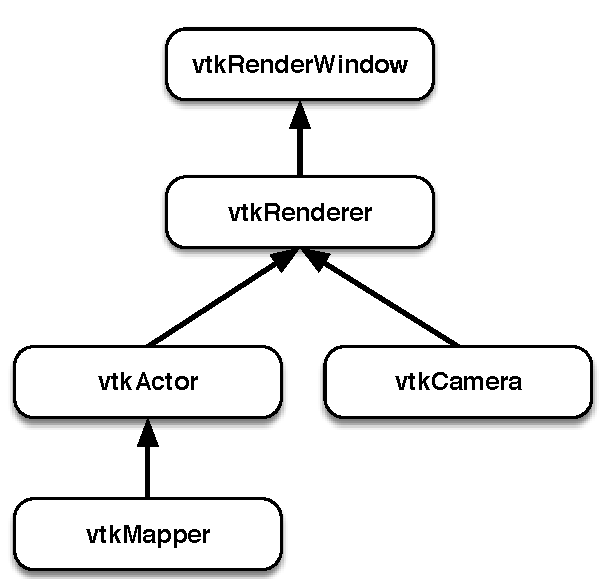
\includegraphics[width=0.5\linewidth]{images/vtkRenderPipeline.pdf}
  \caption{vtkRenderWindow, vtkRenderer, vtkCamera, vtkActor, and vtkMapper interaction diagram.}
  \label{fig:vtkRenderPipeline}
\end{figure}

Since \texttt{vtkRenderWindow} typically creates the context, and \texttt{vtkRenderer} controls the rendering of individual objects in a scene of a given viewport, the rendering pipeline is constructed with properties and other attributes set specifically to support this most general use case.
In the case of external environments, however, the context is created outside of VTK. Non-VTK graphical elements (such as the GUI) may be rendered before or after the VTK rendering.
In addition, the environment may render its own visualization objects in the same context.
To handle this situation, we have introduced a new module in VTK called \texttt{vtkRenderingExternal} that comprises four new classes: \texttt{vtkExternalOpenGLRenderWindow}, \texttt{vtkExternalOpenGLRenderer}, \texttt{vtkExternalOpenGLCamera} and \texttt{ExternalVTKWidget}. 

\textbf{\texttt{vtkExternalOpenGLRenderWindow}} - This class is an extension to
the \texttt{vtkGenericOpenGLRenderWindow} class, which provides a
platform-agnostic VTK OpenGL window.
The external render window class prevents a new VTK render window from being
created and, instead, uses an existing OpenGL context.
It is also responsible for fetching stereo parameters from the parent OpenGL
application and setting them on the VTK pipeline.

\textbf{\texttt{vtkExternalOpenGLRenderer}} - This class derives from
\texttt{vtkRenderer} and provides all of its features and functionalities. The
external renderer offers an API that prevents it from clearing the OpenGL color
and depth buffers at each frame. This ensures that the main application holds
control over the OpenGL context and preserves rendered elements in the scene, of
which VTK is unaware.

\textbf{\texttt{vtkExternalOpenGLCamera}} - This class inherits
\texttt{vtkCamera} and provides the ability to set the projection and modelview
matrices on the camera. This allows the external rendering framework to easily
set the view and orientation on the VTK camera. The external camera also uses
this scene information to compute accurate lighting matrices.

\textbf{\texttt{ExternalVTKWidget}} - This is a collective implementation that
provides a plug-and-play approach to the \texttt{vtkRenderingExternal} module.
It allows the consumer application to use all the new classes as described above
in just one step. The overarching application needs only to instantiate this
class to use VTK's external rendering capabilities. The
\texttt{ExternalVTKWidget} creates a new external render window or uses one
provided to it from the external library/application.

\subsubsection{Implementation}

Some of the most important prerequisites of this work were seamless stereo
rendering and user interaction, between the rendering native to the base VR toolkit and the rendering embedded in VTK. 

\textbf{\textit{Stereo Rendering}} The OpenGL context maintains the state machine, in which OpenGL commands change the state of the system or query a particular state as needed.
To support stereo, we utilized the OpenGL context, set by the VR toolkit, to determine the type of stereo (Quad Buffer, Side-by Side, or Top-Bottom stereo) and simply render using the OpenGL context This context sets the active buffer, stenciling, etc.
Such settings are made only once, immediately after the context has been created, and are maintained by the VR toolkit over time. 

\textbf{\textit{2D and 3D Interface Widgets}} In most cases, VTK elements will not be the only objects in a scene.
There will probably be some GUI elements that will also be rendered in addition to the VTK elements.
Thus, the VTK rendering will be mixed with other OpenGL elements.
The new \texttt{ExternalRenderer} class does not clear the depth or color buffers. It leaves this task to the display integration library or application.
The depth buffer can then act to allow OpenGL elements to be mixed (composited)
in three-dimensional (3D) space, with closer elements occluding farther ones.

\textbf{\textit{User Interactions}} Generally, in the case of a VR toolkit, interactions such as navigation in the scene space, grab, and rotation of various scene objects are handled by the VR integration library (e.g., Vrui).
VTK has its own classes and methods for interaction and scene-object manipulation.
To synchronize the navigation in these two systems, the \texttt{vtkExternalOpenGLCamera} class has been added.
This class empowers the external application to manage camera interaction for VTK objects.
We added a GL query in the external renderer, which uses the GL state system to get the projection and the modelview transformation matrices.
These two matrices determine the location and orientation of the end-user's eye
(camera) in the scene.
The \texttt{vtkExternalOpenGLRenderer} sets these matrices on the \texttt{vtkExternalOpenGLCamera}.
Setting these matrices directly on the camera leaves the camera parameters such as position, focal point, and view-up direction as incorrect values, Therefore, we compute appropriate viewing coordinates for the camera by multiplying the modelview matrix with the camera's initial default position in the OpenGL coordinate system. 
Once, everything is set on the camera, the navigation and lighting works as expected by the end-user.

The application itself handles the secondary kind of interactions such as interactive slicing and clipping of the scientific datasets.
VTK provides classes (filters) to perform thresholding, clipping, slicing, etc.
These filters take parameters such as thresholding value, slicing position and clip position. 
In our implementation, the application receives the 6-DOF tracker position data, and, based on the mode of the application, uses this information to set appropriate values on a specific filter.
For example, the left-hand controller might be used to position the clipping plane.
This integration is straightforward because our module makes the coordinate system consistent between the two rendering systems.

\subsubsection{Enabling \texttt{vtkRenderingExternal}}

This work has been merged into the VTK as of the release of version 7.0, which is available at
\url{http://www.vtk.org}.
To enable this module when compiling VTK with \texttt{CMake},
set \texttt{Module\_vtkRenderingExternal} to \texttt{ON}. (The default is \texttt{OFF}.)

\subsection{VR Toolkit Embedding (Oculus and OpenVR)}

The potential VR user base has grown profusely with the emerging
proliferation of consumer-level HMD VR displays along with their associated
software ecosystems, such as Valve's SteamVR.
For developers who are willing to specifically target this audience, perhaps
excluding users of CAVE-style VR displays, a simpler VTK-VR alternative is
also available.
The trade-off | for developers who don't already have expertise in a
full-fledged VR integration library | is avoiding the programming of
the alternative VR integration library, and immediately gaining access
to HMDs compatible with OpenVR, but not to other VR display systems.

To enable using consumer VR devices with VTK, we created Oculus and OpenVR modules in VTK .
Our goal is to allow VTK programs to use consumer VR devices with few changes, if any, and to support natural interaction when using them.
If the executable is linked to the \texttt{vtkRenderingOpenVR} or \texttt{vtkRenderingOculus} modules, the object factory
mechanism will replace the core rendering classes (e.g.,
\texttt{vtkRenderWindow} and \texttt{vtkRenderer}) with the VR specialized versions in VTK.  This also entails changes to the 
interaction model as VR and VR devices are naturally 3D in nature with single and multi-touch events occurring in 3D space as 
opposed to the more traditional 2D screen space. To this end we created new classes that support natural picking and interaction given 3D 
input devices.

One example of this low barrier of entry is incorporating consumer VR support into the latest release of ParaView. With minimal changes to ParaView we are enabling researchers to load up existing visualizations in ParaView and send them to VR to explore them with the Vive or Rift. Researchers can bounce back and forth between the traditional desktop and consumer VR experiences with the press of a button. This type of integration targets our goal of providing a solution with a low barrier of entry.

\subsubsection{Implementation}

The integrated VR support contains the following classes as drop-in replacements in VTK.

\textbf{\texttt{vtk(OpenVR/Oculus)RenderWindow}} - This is a derived class of the RenderWindow class.
This class holds the initialization and main interfacing to the consumer VR toolkit. 

\textbf{\texttt{vtk(OpenVR/Oculus)Renderer}} - This is a derived class of the Render class.
Consumer VR devices exist in real world coordinates such as meters, while the world coordinate system of a visualization could be anything from microns to AUs. As such, movements in the real world need to be scaled and translated into reasonable movements in the visualization's world coordinates. The \texttt{vtk(OpenVR/Oculus)Renderer} class computes a reasonable scale and translation which are then used in computing the view and input device transforms. 
It also sets an appropriate default clipping range expansion.

\textbf{\texttt{vtk(OpenVR/Oculus)Camera}} - This is a derived class of the Camera class. \texttt{vtk(OpenVR/Oculus)Camera} gets the matrices from the VR library to use for rendering and integrates them with the model, view and world matrices from the visualization. It contains a scale and translation that are designed to map world coordinates into the HMD space.
Accordingly, the application developers can keep world coordinates in the units best suited to their problem domains, and the camera will shift and scale into units that make sense for the HMD.

\textbf{\texttt{vtk(OpenVR/Oculus)RenderWindowInteractor}} - VTK is designed to pick and interact based on two-degrees of freedom, desktop X and Y mouse/window coordinates.
In contrast, VR provides X, Y and Z 3D world coordinates as well as 3D orientations.
The \texttt{vtk(OpenVR/Oculus)RenderWindowInteractor} class catches controller events and converts them to mouse/window events.
In addition, this class also stores the world coordinate positions and orientations for the styles or pickers that need them.
\texttt{vtk(OpenVR/Oculus)RenderWindowInteractor} supports multiple controllers through the standard PointerIndex approach that VTK uses for multi-touch.

\textbf{\texttt{vtkInteractorStyle3D}} - In concert with the VR specialized \texttt{vtkRenderWindowInteractor} classed, we derived the \texttt{vtkInteractorStyle3D} class
to use 3D world coordinate events to manipulate \texttt{Actor}s, and handle multi-touch 3D events such as scaling or translating the world to real transforms.
This class provides a common grab-and-move style of interaction that is common to OpenVR and other VR toolkits.

\textbf{\texttt{vtkPropPicke3D}} - Finally, the derived \texttt{vtkPropPicke3D} class determines what \texttt{Actor}s or \texttt{Prop}s VTK picks.
Note that \texttt{Prop} is an abstract superclass for any object that can exist in a rendered scene (either 2D or 3D). It defines the API for picking; the LOD manipulation; and the common instance variables that control visibility, picking, and dragging.
The \texttt{vtkPropPicker3D} class uses the 3D world coordinate from a VR device as the picking value as opposed to using a 2D event and intersecting a ray, which is slower.

These derived classes work from within VTK to provide seamless access to cameras, lighting, interaction and the complete VTK pipeline.

\subsubsection{Enabling the OpenVR and Oculus Modules}

To use VTK with Oculus or OpenVR support, first download VTK 7.1 or later from the VTK
repository on GitHub (see \url{http://www.vtk.org}).
To enable these modules, use \texttt{CMake} to set \texttt{Module\_vtkRenderingOpenVR} or \texttt{Module\_vtkRenderingOculus} to \texttt{ON}. (The default is \texttt{OFF}.)
The \texttt{CMake} build process will prompt you for some external libraries including Simple DirectMedia Layer 2 (SDL2) and the OpenVR or Oculus SDK as appropriate.
Ensure to build an optimized version of VTK to maximize performance while using these new capabilities.

\subsubsection{Future Developments}

The consumer VR support is currently in the beta phase and has been tested on the HTC Vive and Oculus Rift. Moving forward, we look to add support for the features such as overlays, which provide support for user interface components. We also expect to include more event interactions, Oculus touch controller support, and measurement widgets.

\subsection{Performance enhancements}

VTK is one of the most commonly used libraries for visualization and computation in the scientific community.
Primarily written in C++, VTK provides classical and model visualization algorithms to visualize structured, unstructured, and point data sets on desktop, mobile, and web environments.
VTK provides state-of-the-art implementations that are accessible via an API call.
The benefit of using VTK comes from the fact that having the latest algorithm implementation simply requires using the existing implementation from the
open-source, community-driven VTK repository or contributing one.

To allow VTK to function at levels needed for head-tracked rendering,
many other enhancements have been added to the overall VTK system:
using modern OpenGL,
rendering transparencies with dual-depth peeling, and
expanding the use of multi-threading.

\subsubsection{OpenGL 3.2+}

The legacy rendering code in VTK is a group of implementation modules collectively called ``OpenGL."
Through a grant from the National Institutes of Health, the OpenGL group has
been rewritten as a drop-in replacement set of implementation modules
collectively called ``OpenGL2".
This work aims to support rendering on modern graphics cards~\cite{Hanwell:2015}.

The results have been nothing short of spectacular.
Polygon rendering demonstrates a tenfold speed-up for the first frame rendering, followed by a two-hundredfold speed-up for subsequent frames for upto thirty million triangles.
The previous volume rendering was also graphics processing unit (GPU) aware, and, thus, the improvement is a modest but substantial two fold speed-up. 

To realize these performance enhancements, VTK now uses an OpenGL 3.2+ context, which is available on fairly low-end modern GPUs.
For those application developers using the X11 window system on a Mac OSX system, xQuartz does not currently provide a suitable OpenGL context.
As xQuatrz utilizes newer versions of Mesa going forward, we expect future versions will eventually meet the OpenGL2 requirements.

\subsubsection{Dual-Depth Peeling}

As we developed several example programs that leverage the \texttt{vtkRenderingExternal} module, we found that the rendering performance slowed as transparency was introduced into the scene. We have developed a dual-depth peeling algorithm to overcome this issue.

In OpenGL, polygons are broken up into fragments through the rasterization process.
Each fragment corresponds to a pixel.
An OpenGL fragment shader is a customizable program that determines the color of a fragment where all fragments for a single pixel are blended to determine the final color of the pixel.
Composing multiple translucent fragments into a single pixel must be done carefully.
There are three common strategies to this composition:

\begin{compactitem}
\item \textbf{Simple Alpha Blending} - Fragments are processed (blended using just alpha) in random order.
  It is very fast, but it provides unpredictable and generally incorrect results.
\item \textbf{Sorted Geometry} - Geometry must be resorted each time the camera moves using \texttt{vtkDepthSortPolyData}.
  Sorting is an expensive (slow) operation, but it provides generally consistent results with some artifacts where primitives overlap.
\item \textbf{Depth Peeling} - Fragments are extracted and blended in a multipass render. Therefore, the process requires multiple geometry render passes.
\end{compactitem}

VTK by default uses depth peeling.
To enhance rendering performance with transparency we implemented \texttt{vtkDualDepthPeelingPass}, which was originally proposed by nVidia in 2008~\cite{Bavoil:2008}.
Dual-depth peeling extends traditional depth peeling by extracting two layers of fragments per-pass: from the front and back simultaneously.
It uses a two-component depth buffer to track of peel information and three types of geometry passes:

\begin{compactitem}
\item \textbf{InitializeDepth} - A pass that initializes buffers using opaque geometry information.
\item \textbf{Peeling} - A repeated pass that extracts and blends translucent geometry peels. It extracts both near and far peels while blending far peels into the accumulation buffer.
\item \textbf{AlphaBlending} - An optional pass to clean up unpeeled fragments that are used with occlusion thresholds.
\end{compactitem}

This algorithm provides a two fold speed-up for compositing in the appearance of transparent geometry.

\subsubsection{vtkSMPTools}

The field of parallel computing is advancing rapidly due to innovations in GPU and multicore technologies.
The VTK community is working to make parallel computing for scientific visualization easier by introducing \texttt{vtkSMPTools}, an abstraction for threaded processing which uses different libraries such as TBB~\cite{TBB:2016}, OpenMP~\cite{OpenMP:2016} and XKaapi~\cite{Gautier:2013}.
The typical target application is coarse-grained shared-memory computing as provided by mainstream multicore, threaded CPUs such as Intel's i5 and i7 architectures.

For several of the example programs, that utilize the \texttt{vtkRenderingExternal} module, we leveraged a new contouring algorithms in VTK that are readily parallelizable using \texttt{vtkSMPTools} and still incredibly efficient in serial mode, called \texttt{vtkFlyingEdges2D} and \texttt{vtkFlyingEdges3D}.
While the OpenGL2 group improves rendering performance, \texttt{vtkSMPTools} can be used to enhance the geometry generation performance for scientific visualization.
